\chapter{Introduction}
\subsection{abstract}
The acceptance of service robots comes along with the ability to adapt to user specific preferences. This requires that a robot can determine the identity of the user. As for humans, robust user recognition is based on the identification of the face. However, despite the plethora of published work on face recognition that is robust against real world noise such a illumination, head alignment or facial expressions there is no robust off-the-shelf non-commercial software available to be used in typical robotics applications. Hence, this paper introduces a ready-to-use open-source ROS package providing a face detection and identification system that is comprising novel and state-of-the-art solutions to various aspects of face recognition while utilizing modern RGB-D sensors. This work demonstrates a solution for face recognition in robotic settings that is robust against varying illumination, gaze directions of the head, and facial expressions while operating with online performance. The paper provides a thorough evaluation of the face recognition system based on standard database tests and on real world scenarios regarding these criteria.


%%%%%%%%%%%%%%%%%%%%%%%%%%%%%%%%%%%%%%%%%%%%%%%%%%%%%%%%%%%%%%%%%%%%%%%%%%%%%%%%
\section{Introduction}
%- 1 Paragraph general introduction to robotics, face recognition, applications
%- 1 Paragraph concrete problem and subproblems tackled in the paper
%- we need a reference to our covergirl image somewhere in these paragraphs

With service robots becoming more and more capable of doing useful work in households appropriate user interaction becomes increasingly important. For example, in the EU-funded project Accompany we are researching how a multifunctional service robot like Care-O-bot 3 may assist elderly persons with their daily activities, like transporting items, delivery tasks, reminder functions, or grasping objects from a shelf. Such services and the interaction with the user therein are highly user specific and the robot is required to interact with multiple kinds of users in the respective ways. Hence, the identification of individual users is a crucial precondition to successful interaction.

Despite this apparent need for accurate user identification in applications for service robots there are, besides many commercial solutions, only few open-source systems available. The most prominent examples are libface \cite{jironkin2010} and the ROS stack people \cite{pantofaru2010}, which both use the Viola-Jones classifier \cite{Viola01} for face detection and Eigenfaces \cite{Turk1991} for recognition, as well as OpenCV \cite{bradski2008} itself which has been enhanced by several modern recognition algorithms recently. However, although there is a large body of research dedicated to person recognition under difficult circumstances such as varying illumination, head pose, or facial expressions, robotics could not benefit from a ready-to-use solution so far which covers all the challenges occurring in real operation. Hence, the motivation for this work was to develop a complete person identification pipeline that exploits the benefits of RGB-D streams from inexpensive RGB-D cameras and that is insensitive to typical real-world influences such as illumination, head pose, and facial expressions, while maintaining online performance for usage with real robots. Moreover, the system should be able to safely distinguish at least 30 people, detect unknown people as being new, and unknown subjects should be easily and quickly added to the database without any fancy requirements regarding the recording settings for the sample face images.

%- OpenCV provides some algorithms for detection and recognition
%- libface - uses OpenCV detection and implements Eigenfaces
%- people stack

%motivation:
%- ready-to-use person identification pipeline
%- uses RGB-D image streams
%- insensitive to typical real-world influences as illumination, head pose, facial expressions
%- real-time performance
%- quickly trainable in any situation (no fixed recording procedure or defined lighting necessary, few training images), fast integration of new training data to recognition module
%- possibility to detect unknown people as being new
%- safely distinguishing numbers up to 30 people

\begin{figure}[t]
	\begin{center}
		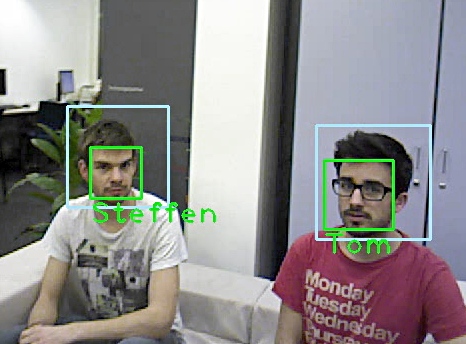
\includegraphics[width=0.76\columnwidth]{title_image.png}
	\end{center}
	\caption{Head detection (blue frame), face detection (green frame) and recognition of identity in real world service robotics applications.} \vspace{-2mm}
	\label{fig:covergirl}
\end{figure}

This paper introduces a person identification system that combines face detection based on our previous work \cite{Fischer2010}, modern preprocessing procedures and face recognition based on Fisherfaces \cite{Belhumeur1997} as well as a tracking system for continuous and robust identification of persons in RGB-D image streams. The whole system fulfills all of the mentioned requirements making it ready for the use with a real service robot. The main contributions of this work are:
\begin{enumerate}
	\item A ready-to-use open-source ROS package\footnote{the software is available as \texttt{cob\_people\_perception} stack at \url{http://www.ros.org/wiki/cob_people_perception}} providing a complete face detection and identification system that is well-suited for application in robotics domains.
	\item A combination of novel and state-of-the-art methods for RGB-D face recognition selected on the basis of a thorough literature review.
	\item A comprehensive evaluation of the face recognition system regarding the imposed criteria.
\end{enumerate}
%Highlight that our experiments prove that our implementation fulfills all these requirements achieving high recognition rates under the considered perturbations using always a small and not diverse set of training images for all tests.
%This paper discusses our follow-up work to \cite{Fischer2010} where the face detection system has been described in detail. 

The remainder of this paper is structured as follows. After a discussion of relevant work in Sec. \ref{sec:relatedwork} the utilized algorithms are explained in Sec. \ref{sec:methods}. Following the face recognition system is evaluated in Sec. \ref{sec:evaluation} with regard to accuracy and robustness aspects. The paper concludes with a summary and an outlook for following research in Sec. \ref{sec:conclusions}.
